
% Default to the notebook output style

    


% Inherit from the specified cell style.




    
\documentclass[11pt]{article}

    
    
    \usepackage[T1]{fontenc}
    % Nicer default font (+ math font) than Computer Modern for most use cases
    \usepackage{mathpazo}

    % Basic figure setup, for now with no caption control since it's done
    % automatically by Pandoc (which extracts ![](path) syntax from Markdown).
    \usepackage{graphicx}
    % We will generate all images so they have a width \maxwidth. This means
    % that they will get their normal width if they fit onto the page, but
    % are scaled down if they would overflow the margins.
    \makeatletter
    \def\maxwidth{\ifdim\Gin@nat@width>\linewidth\linewidth
    \else\Gin@nat@width\fi}
    \makeatother
    \let\Oldincludegraphics\includegraphics
    % Set max figure width to be 80% of text width, for now hardcoded.
    \renewcommand{\includegraphics}[1]{\Oldincludegraphics[width=.8\maxwidth]{#1}}
    % Ensure that by default, figures have no caption (until we provide a
    % proper Figure object with a Caption API and a way to capture that
    % in the conversion process - todo).
    \usepackage{caption}
    \DeclareCaptionLabelFormat{nolabel}{}
    \captionsetup{labelformat=nolabel}

    \usepackage{adjustbox} % Used to constrain images to a maximum size 
    \usepackage{xcolor} % Allow colors to be defined
    \usepackage{enumerate} % Needed for markdown enumerations to work
    \usepackage{geometry} % Used to adjust the document margins
    \usepackage{amsmath} % Equations
    \usepackage{amssymb} % Equations
    \usepackage{textcomp} % defines textquotesingle
    % Hack from http://tex.stackexchange.com/a/47451/13684:
    \AtBeginDocument{%
        \def\PYZsq{\textquotesingle}% Upright quotes in Pygmentized code
    }
    \usepackage{upquote} % Upright quotes for verbatim code
    \usepackage{eurosym} % defines \euro
    \usepackage[mathletters]{ucs} % Extended unicode (utf-8) support
    \usepackage[utf8x]{inputenc} % Allow utf-8 characters in the tex document
    \usepackage{fancyvrb} % verbatim replacement that allows latex
    \usepackage{grffile} % extends the file name processing of package graphics 
                         % to support a larger range 
    % The hyperref package gives us a pdf with properly built
    % internal navigation ('pdf bookmarks' for the table of contents,
    % internal cross-reference links, web links for URLs, etc.)
    \usepackage{hyperref}
    \usepackage{longtable} % longtable support required by pandoc >1.10
    \usepackage{booktabs}  % table support for pandoc > 1.12.2
    \usepackage[inline]{enumitem} % IRkernel/repr support (it uses the enumerate* environment)
    \usepackage[normalem]{ulem} % ulem is needed to support strikethroughs (\sout)
                                % normalem makes italics be italics, not underlines
    

    
    
    % Colors for the hyperref package
    \definecolor{urlcolor}{rgb}{0,.145,.698}
    \definecolor{linkcolor}{rgb}{.71,0.21,0.01}
    \definecolor{citecolor}{rgb}{.12,.54,.11}

    % ANSI colors
    \definecolor{ansi-black}{HTML}{3E424D}
    \definecolor{ansi-black-intense}{HTML}{282C36}
    \definecolor{ansi-red}{HTML}{E75C58}
    \definecolor{ansi-red-intense}{HTML}{B22B31}
    \definecolor{ansi-green}{HTML}{00A250}
    \definecolor{ansi-green-intense}{HTML}{007427}
    \definecolor{ansi-yellow}{HTML}{DDB62B}
    \definecolor{ansi-yellow-intense}{HTML}{B27D12}
    \definecolor{ansi-blue}{HTML}{208FFB}
    \definecolor{ansi-blue-intense}{HTML}{0065CA}
    \definecolor{ansi-magenta}{HTML}{D160C4}
    \definecolor{ansi-magenta-intense}{HTML}{A03196}
    \definecolor{ansi-cyan}{HTML}{60C6C8}
    \definecolor{ansi-cyan-intense}{HTML}{258F8F}
    \definecolor{ansi-white}{HTML}{C5C1B4}
    \definecolor{ansi-white-intense}{HTML}{A1A6B2}

    % commands and environments needed by pandoc snippets
    % extracted from the output of `pandoc -s`
    \providecommand{\tightlist}{%
      \setlength{\itemsep}{0pt}\setlength{\parskip}{0pt}}
    \DefineVerbatimEnvironment{Highlighting}{Verbatim}{commandchars=\\\{\}}
    % Add ',fontsize=\small' for more characters per line
    \newenvironment{Shaded}{}{}
    \newcommand{\KeywordTok}[1]{\textcolor[rgb]{0.00,0.44,0.13}{\textbf{{#1}}}}
    \newcommand{\DataTypeTok}[1]{\textcolor[rgb]{0.56,0.13,0.00}{{#1}}}
    \newcommand{\DecValTok}[1]{\textcolor[rgb]{0.25,0.63,0.44}{{#1}}}
    \newcommand{\BaseNTok}[1]{\textcolor[rgb]{0.25,0.63,0.44}{{#1}}}
    \newcommand{\FloatTok}[1]{\textcolor[rgb]{0.25,0.63,0.44}{{#1}}}
    \newcommand{\CharTok}[1]{\textcolor[rgb]{0.25,0.44,0.63}{{#1}}}
    \newcommand{\StringTok}[1]{\textcolor[rgb]{0.25,0.44,0.63}{{#1}}}
    \newcommand{\CommentTok}[1]{\textcolor[rgb]{0.38,0.63,0.69}{\textit{{#1}}}}
    \newcommand{\OtherTok}[1]{\textcolor[rgb]{0.00,0.44,0.13}{{#1}}}
    \newcommand{\AlertTok}[1]{\textcolor[rgb]{1.00,0.00,0.00}{\textbf{{#1}}}}
    \newcommand{\FunctionTok}[1]{\textcolor[rgb]{0.02,0.16,0.49}{{#1}}}
    \newcommand{\RegionMarkerTok}[1]{{#1}}
    \newcommand{\ErrorTok}[1]{\textcolor[rgb]{1.00,0.00,0.00}{\textbf{{#1}}}}
    \newcommand{\NormalTok}[1]{{#1}}
    
    % Additional commands for more recent versions of Pandoc
    \newcommand{\ConstantTok}[1]{\textcolor[rgb]{0.53,0.00,0.00}{{#1}}}
    \newcommand{\SpecialCharTok}[1]{\textcolor[rgb]{0.25,0.44,0.63}{{#1}}}
    \newcommand{\VerbatimStringTok}[1]{\textcolor[rgb]{0.25,0.44,0.63}{{#1}}}
    \newcommand{\SpecialStringTok}[1]{\textcolor[rgb]{0.73,0.40,0.53}{{#1}}}
    \newcommand{\ImportTok}[1]{{#1}}
    \newcommand{\DocumentationTok}[1]{\textcolor[rgb]{0.73,0.13,0.13}{\textit{{#1}}}}
    \newcommand{\AnnotationTok}[1]{\textcolor[rgb]{0.38,0.63,0.69}{\textbf{\textit{{#1}}}}}
    \newcommand{\CommentVarTok}[1]{\textcolor[rgb]{0.38,0.63,0.69}{\textbf{\textit{{#1}}}}}
    \newcommand{\VariableTok}[1]{\textcolor[rgb]{0.10,0.09,0.49}{{#1}}}
    \newcommand{\ControlFlowTok}[1]{\textcolor[rgb]{0.00,0.44,0.13}{\textbf{{#1}}}}
    \newcommand{\OperatorTok}[1]{\textcolor[rgb]{0.40,0.40,0.40}{{#1}}}
    \newcommand{\BuiltInTok}[1]{{#1}}
    \newcommand{\ExtensionTok}[1]{{#1}}
    \newcommand{\PreprocessorTok}[1]{\textcolor[rgb]{0.74,0.48,0.00}{{#1}}}
    \newcommand{\AttributeTok}[1]{\textcolor[rgb]{0.49,0.56,0.16}{{#1}}}
    \newcommand{\InformationTok}[1]{\textcolor[rgb]{0.38,0.63,0.69}{\textbf{\textit{{#1}}}}}
    \newcommand{\WarningTok}[1]{\textcolor[rgb]{0.38,0.63,0.69}{\textbf{\textit{{#1}}}}}
    
    
    % Define a nice break command that doesn't care if a line doesn't already
    % exist.
    \def\br{\hspace*{\fill} \\* }
    % Math Jax compatability definitions
    \def\gt{>}
    \def\lt{<}
    % Document parameters
    \title{RL-Quadcopter}
    
    
    

    % Pygments definitions
    
\makeatletter
\def\PY@reset{\let\PY@it=\relax \let\PY@bf=\relax%
    \let\PY@ul=\relax \let\PY@tc=\relax%
    \let\PY@bc=\relax \let\PY@ff=\relax}
\def\PY@tok#1{\csname PY@tok@#1\endcsname}
\def\PY@toks#1+{\ifx\relax#1\empty\else%
    \PY@tok{#1}\expandafter\PY@toks\fi}
\def\PY@do#1{\PY@bc{\PY@tc{\PY@ul{%
    \PY@it{\PY@bf{\PY@ff{#1}}}}}}}
\def\PY#1#2{\PY@reset\PY@toks#1+\relax+\PY@do{#2}}

\expandafter\def\csname PY@tok@w\endcsname{\def\PY@tc##1{\textcolor[rgb]{0.73,0.73,0.73}{##1}}}
\expandafter\def\csname PY@tok@c\endcsname{\let\PY@it=\textit\def\PY@tc##1{\textcolor[rgb]{0.25,0.50,0.50}{##1}}}
\expandafter\def\csname PY@tok@cp\endcsname{\def\PY@tc##1{\textcolor[rgb]{0.74,0.48,0.00}{##1}}}
\expandafter\def\csname PY@tok@k\endcsname{\let\PY@bf=\textbf\def\PY@tc##1{\textcolor[rgb]{0.00,0.50,0.00}{##1}}}
\expandafter\def\csname PY@tok@kp\endcsname{\def\PY@tc##1{\textcolor[rgb]{0.00,0.50,0.00}{##1}}}
\expandafter\def\csname PY@tok@kt\endcsname{\def\PY@tc##1{\textcolor[rgb]{0.69,0.00,0.25}{##1}}}
\expandafter\def\csname PY@tok@o\endcsname{\def\PY@tc##1{\textcolor[rgb]{0.40,0.40,0.40}{##1}}}
\expandafter\def\csname PY@tok@ow\endcsname{\let\PY@bf=\textbf\def\PY@tc##1{\textcolor[rgb]{0.67,0.13,1.00}{##1}}}
\expandafter\def\csname PY@tok@nb\endcsname{\def\PY@tc##1{\textcolor[rgb]{0.00,0.50,0.00}{##1}}}
\expandafter\def\csname PY@tok@nf\endcsname{\def\PY@tc##1{\textcolor[rgb]{0.00,0.00,1.00}{##1}}}
\expandafter\def\csname PY@tok@nc\endcsname{\let\PY@bf=\textbf\def\PY@tc##1{\textcolor[rgb]{0.00,0.00,1.00}{##1}}}
\expandafter\def\csname PY@tok@nn\endcsname{\let\PY@bf=\textbf\def\PY@tc##1{\textcolor[rgb]{0.00,0.00,1.00}{##1}}}
\expandafter\def\csname PY@tok@ne\endcsname{\let\PY@bf=\textbf\def\PY@tc##1{\textcolor[rgb]{0.82,0.25,0.23}{##1}}}
\expandafter\def\csname PY@tok@nv\endcsname{\def\PY@tc##1{\textcolor[rgb]{0.10,0.09,0.49}{##1}}}
\expandafter\def\csname PY@tok@no\endcsname{\def\PY@tc##1{\textcolor[rgb]{0.53,0.00,0.00}{##1}}}
\expandafter\def\csname PY@tok@nl\endcsname{\def\PY@tc##1{\textcolor[rgb]{0.63,0.63,0.00}{##1}}}
\expandafter\def\csname PY@tok@ni\endcsname{\let\PY@bf=\textbf\def\PY@tc##1{\textcolor[rgb]{0.60,0.60,0.60}{##1}}}
\expandafter\def\csname PY@tok@na\endcsname{\def\PY@tc##1{\textcolor[rgb]{0.49,0.56,0.16}{##1}}}
\expandafter\def\csname PY@tok@nt\endcsname{\let\PY@bf=\textbf\def\PY@tc##1{\textcolor[rgb]{0.00,0.50,0.00}{##1}}}
\expandafter\def\csname PY@tok@nd\endcsname{\def\PY@tc##1{\textcolor[rgb]{0.67,0.13,1.00}{##1}}}
\expandafter\def\csname PY@tok@s\endcsname{\def\PY@tc##1{\textcolor[rgb]{0.73,0.13,0.13}{##1}}}
\expandafter\def\csname PY@tok@sd\endcsname{\let\PY@it=\textit\def\PY@tc##1{\textcolor[rgb]{0.73,0.13,0.13}{##1}}}
\expandafter\def\csname PY@tok@si\endcsname{\let\PY@bf=\textbf\def\PY@tc##1{\textcolor[rgb]{0.73,0.40,0.53}{##1}}}
\expandafter\def\csname PY@tok@se\endcsname{\let\PY@bf=\textbf\def\PY@tc##1{\textcolor[rgb]{0.73,0.40,0.13}{##1}}}
\expandafter\def\csname PY@tok@sr\endcsname{\def\PY@tc##1{\textcolor[rgb]{0.73,0.40,0.53}{##1}}}
\expandafter\def\csname PY@tok@ss\endcsname{\def\PY@tc##1{\textcolor[rgb]{0.10,0.09,0.49}{##1}}}
\expandafter\def\csname PY@tok@sx\endcsname{\def\PY@tc##1{\textcolor[rgb]{0.00,0.50,0.00}{##1}}}
\expandafter\def\csname PY@tok@m\endcsname{\def\PY@tc##1{\textcolor[rgb]{0.40,0.40,0.40}{##1}}}
\expandafter\def\csname PY@tok@gh\endcsname{\let\PY@bf=\textbf\def\PY@tc##1{\textcolor[rgb]{0.00,0.00,0.50}{##1}}}
\expandafter\def\csname PY@tok@gu\endcsname{\let\PY@bf=\textbf\def\PY@tc##1{\textcolor[rgb]{0.50,0.00,0.50}{##1}}}
\expandafter\def\csname PY@tok@gd\endcsname{\def\PY@tc##1{\textcolor[rgb]{0.63,0.00,0.00}{##1}}}
\expandafter\def\csname PY@tok@gi\endcsname{\def\PY@tc##1{\textcolor[rgb]{0.00,0.63,0.00}{##1}}}
\expandafter\def\csname PY@tok@gr\endcsname{\def\PY@tc##1{\textcolor[rgb]{1.00,0.00,0.00}{##1}}}
\expandafter\def\csname PY@tok@ge\endcsname{\let\PY@it=\textit}
\expandafter\def\csname PY@tok@gs\endcsname{\let\PY@bf=\textbf}
\expandafter\def\csname PY@tok@gp\endcsname{\let\PY@bf=\textbf\def\PY@tc##1{\textcolor[rgb]{0.00,0.00,0.50}{##1}}}
\expandafter\def\csname PY@tok@go\endcsname{\def\PY@tc##1{\textcolor[rgb]{0.53,0.53,0.53}{##1}}}
\expandafter\def\csname PY@tok@gt\endcsname{\def\PY@tc##1{\textcolor[rgb]{0.00,0.27,0.87}{##1}}}
\expandafter\def\csname PY@tok@err\endcsname{\def\PY@bc##1{\setlength{\fboxsep}{0pt}\fcolorbox[rgb]{1.00,0.00,0.00}{1,1,1}{\strut ##1}}}
\expandafter\def\csname PY@tok@kc\endcsname{\let\PY@bf=\textbf\def\PY@tc##1{\textcolor[rgb]{0.00,0.50,0.00}{##1}}}
\expandafter\def\csname PY@tok@kd\endcsname{\let\PY@bf=\textbf\def\PY@tc##1{\textcolor[rgb]{0.00,0.50,0.00}{##1}}}
\expandafter\def\csname PY@tok@kn\endcsname{\let\PY@bf=\textbf\def\PY@tc##1{\textcolor[rgb]{0.00,0.50,0.00}{##1}}}
\expandafter\def\csname PY@tok@kr\endcsname{\let\PY@bf=\textbf\def\PY@tc##1{\textcolor[rgb]{0.00,0.50,0.00}{##1}}}
\expandafter\def\csname PY@tok@bp\endcsname{\def\PY@tc##1{\textcolor[rgb]{0.00,0.50,0.00}{##1}}}
\expandafter\def\csname PY@tok@fm\endcsname{\def\PY@tc##1{\textcolor[rgb]{0.00,0.00,1.00}{##1}}}
\expandafter\def\csname PY@tok@vc\endcsname{\def\PY@tc##1{\textcolor[rgb]{0.10,0.09,0.49}{##1}}}
\expandafter\def\csname PY@tok@vg\endcsname{\def\PY@tc##1{\textcolor[rgb]{0.10,0.09,0.49}{##1}}}
\expandafter\def\csname PY@tok@vi\endcsname{\def\PY@tc##1{\textcolor[rgb]{0.10,0.09,0.49}{##1}}}
\expandafter\def\csname PY@tok@vm\endcsname{\def\PY@tc##1{\textcolor[rgb]{0.10,0.09,0.49}{##1}}}
\expandafter\def\csname PY@tok@sa\endcsname{\def\PY@tc##1{\textcolor[rgb]{0.73,0.13,0.13}{##1}}}
\expandafter\def\csname PY@tok@sb\endcsname{\def\PY@tc##1{\textcolor[rgb]{0.73,0.13,0.13}{##1}}}
\expandafter\def\csname PY@tok@sc\endcsname{\def\PY@tc##1{\textcolor[rgb]{0.73,0.13,0.13}{##1}}}
\expandafter\def\csname PY@tok@dl\endcsname{\def\PY@tc##1{\textcolor[rgb]{0.73,0.13,0.13}{##1}}}
\expandafter\def\csname PY@tok@s2\endcsname{\def\PY@tc##1{\textcolor[rgb]{0.73,0.13,0.13}{##1}}}
\expandafter\def\csname PY@tok@sh\endcsname{\def\PY@tc##1{\textcolor[rgb]{0.73,0.13,0.13}{##1}}}
\expandafter\def\csname PY@tok@s1\endcsname{\def\PY@tc##1{\textcolor[rgb]{0.73,0.13,0.13}{##1}}}
\expandafter\def\csname PY@tok@mb\endcsname{\def\PY@tc##1{\textcolor[rgb]{0.40,0.40,0.40}{##1}}}
\expandafter\def\csname PY@tok@mf\endcsname{\def\PY@tc##1{\textcolor[rgb]{0.40,0.40,0.40}{##1}}}
\expandafter\def\csname PY@tok@mh\endcsname{\def\PY@tc##1{\textcolor[rgb]{0.40,0.40,0.40}{##1}}}
\expandafter\def\csname PY@tok@mi\endcsname{\def\PY@tc##1{\textcolor[rgb]{0.40,0.40,0.40}{##1}}}
\expandafter\def\csname PY@tok@il\endcsname{\def\PY@tc##1{\textcolor[rgb]{0.40,0.40,0.40}{##1}}}
\expandafter\def\csname PY@tok@mo\endcsname{\def\PY@tc##1{\textcolor[rgb]{0.40,0.40,0.40}{##1}}}
\expandafter\def\csname PY@tok@ch\endcsname{\let\PY@it=\textit\def\PY@tc##1{\textcolor[rgb]{0.25,0.50,0.50}{##1}}}
\expandafter\def\csname PY@tok@cm\endcsname{\let\PY@it=\textit\def\PY@tc##1{\textcolor[rgb]{0.25,0.50,0.50}{##1}}}
\expandafter\def\csname PY@tok@cpf\endcsname{\let\PY@it=\textit\def\PY@tc##1{\textcolor[rgb]{0.25,0.50,0.50}{##1}}}
\expandafter\def\csname PY@tok@c1\endcsname{\let\PY@it=\textit\def\PY@tc##1{\textcolor[rgb]{0.25,0.50,0.50}{##1}}}
\expandafter\def\csname PY@tok@cs\endcsname{\let\PY@it=\textit\def\PY@tc##1{\textcolor[rgb]{0.25,0.50,0.50}{##1}}}

\def\PYZbs{\char`\\}
\def\PYZus{\char`\_}
\def\PYZob{\char`\{}
\def\PYZcb{\char`\}}
\def\PYZca{\char`\^}
\def\PYZam{\char`\&}
\def\PYZlt{\char`\<}
\def\PYZgt{\char`\>}
\def\PYZsh{\char`\#}
\def\PYZpc{\char`\%}
\def\PYZdl{\char`\$}
\def\PYZhy{\char`\-}
\def\PYZsq{\char`\'}
\def\PYZdq{\char`\"}
\def\PYZti{\char`\~}
% for compatibility with earlier versions
\def\PYZat{@}
\def\PYZlb{[}
\def\PYZrb{]}
\makeatother


    % Exact colors from NB
    \definecolor{incolor}{rgb}{0.0, 0.0, 0.5}
    \definecolor{outcolor}{rgb}{0.545, 0.0, 0.0}



    
    % Prevent overflowing lines due to hard-to-break entities
    \sloppy 
    % Setup hyperref package
    \hypersetup{
      breaklinks=true,  % so long urls are correctly broken across lines
      colorlinks=true,
      urlcolor=urlcolor,
      linkcolor=linkcolor,
      citecolor=citecolor,
      }
    % Slightly bigger margins than the latex defaults
    
    \geometry{verbose,tmargin=1in,bmargin=1in,lmargin=1in,rmargin=1in}
    
    

    \begin{document}
    
    
    \maketitle
    
    

    
    \section{Project: Train a Quadcopter How to
Fly}\label{project-train-a-quadcopter-how-to-fly}

Design an agent that can fly a quadcopter, and then train it using a
reinforcement learning algorithm of your choice! Try to apply the
techniques you have learnt, but also feel free to come up with
innovative ideas and test them.

\begin{figure}
\centering
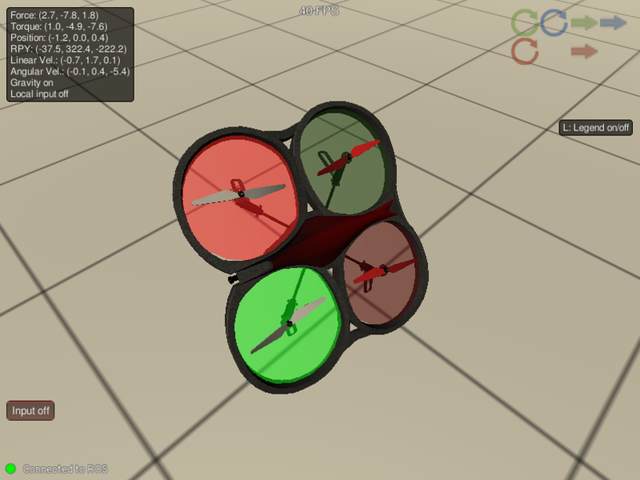
\includegraphics{images/quadcopter_tumble.png}
\caption{Quadcopter doing a flip trying to takeoff from the ground}
\end{figure}

\subsection{Instructions}\label{instructions}

\begin{quote}
\textbf{Note}: If you haven't done so already, follow the steps in this
repo's README to install ROS, and ensure that the simulator is running
and correctly connecting to ROS.
\end{quote}

When you are ready to start coding, take a look at the
\texttt{quad\_controller\_rl/src/} (source) directory to better
understand the structure. Here are some of the salient items:

\begin{itemize}
\tightlist
\item
  \texttt{src/}: Contains all the source code for the project.
\item
  \texttt{quad\_controller\_rl/}: This is the root of the Python package
  you'll be working in.
\item
  ...
\item
  \texttt{tasks/}: Define your tasks (environments) in this
  sub-directory.

  \begin{itemize}
  \tightlist
  \item
    \texttt{\_\_init\_\_.py}: When you define a new task, you'll have to
    import it here.
  \item
    \texttt{base\_task.py}: Generic base class for all tasks, with
    documentation.
  \item
    \texttt{takeoff.py}: This is the first task, already defined for
    you, and set to run by default.
  \end{itemize}
\item
  ...
\item
  \texttt{agents/}: Develop your reinforcement learning agents here.

  \begin{itemize}
  \tightlist
  \item
    \texttt{\_\_init\_\_.py}: When you define a new agent, you'll have
    to import it here, just like tasks.
  \item
    \texttt{base\_agent.py}: Generic base class for all agents, with
    documentation.
  \item
    \texttt{policy\_search.py}: A sample agent has been provided here,
    and is set to run by default.
  \end{itemize}
\item
  ...
\end{itemize}

\subsubsection{Tasks}\label{tasks}

Open up the base class for tasks, \texttt{BaseTask}, defined in
\texttt{tasks/base\_task.py}:

\begin{Shaded}
\begin{Highlighting}[]
\KeywordTok{class}\NormalTok{ BaseTask:}
    \CommentTok{"""Generic base class for reinforcement learning tasks."""}

    \KeywordTok{def} \FunctionTok{__init__}\NormalTok{(}\VariableTok{self}\NormalTok{):}
        \CommentTok{"""Define state and action spaces, initialize other task parameters."""}
        \ControlFlowTok{pass}
    
    \KeywordTok{def}\NormalTok{ set_agent(}\VariableTok{self}\NormalTok{, agent):}
        \CommentTok{"""Set an agent to carry out this task; to be called from update."""}
        \VariableTok{self}\NormalTok{.agent }\OperatorTok{=}\NormalTok{ agent}
    
    \KeywordTok{def}\NormalTok{ reset(}\VariableTok{self}\NormalTok{):}
        \CommentTok{"""Reset task and return initial condition."""}
        \ControlFlowTok{raise} \PreprocessorTok{NotImplementedError}
    
    \KeywordTok{def}\NormalTok{ update(}\VariableTok{self}\NormalTok{, timestamp, pose, angular_velocity, linear_acceleration):}
        \CommentTok{"""Process current data, call agent, return action and done flag."""}
        \ControlFlowTok{raise} \PreprocessorTok{NotImplementedError}            
\end{Highlighting}
\end{Shaded}

All tasks must inherit from this class to function properly. You will
need to override the \texttt{reset()} and \texttt{update()} methods when
defining a task, otherwise you will get \texttt{NotImplementedError}'s.
Besides these two, you should define the state (observation) space and
the action space for the task in the constructor,
\texttt{\_\_init\_\_()}, and initialize any other variables you may need
to run the task.

Now compare this with the first concrete task \texttt{Takeoff}, defined
in \texttt{tasks/takeoff.py}:

\begin{Shaded}
\begin{Highlighting}[]
\KeywordTok{class}\NormalTok{ Takeoff(BaseTask):}
    \CommentTok{"""Simple task where the goal is to lift off the ground and reach a target height."""}
\NormalTok{    ...}
\end{Highlighting}
\end{Shaded}

In \texttt{\_\_init\_\_()}, notice how the state and action spaces are
defined using \href{https://gym.openai.com/docs/\#spaces}{OpenAI Gym
spaces}, like
\href{https://github.com/openai/gym/blob/master/gym/spaces/box.py}{\texttt{Box}}.
These objects provide a clean and powerful interface for agents to
explore. For instance, they can inspect the dimensionality of a space
(\texttt{shape}), ask for the limits (\texttt{high} and \texttt{low}),
or even sample a bunch of observations using the \texttt{sample()}
method, before beginning to interact with the environment. We also set a
time limit (\texttt{max\_duration}) for each episode here, and the
height (\texttt{target\_z}) that the quadcopter needs to reach for a
successful takeoff.

The \texttt{reset()} method is meant to give you a chance to
reset/initialize any variables you need in order to prepare for the next
episode. You do not need to call it yourself; it will be invoked
externally. And yes, it will be called once before each episode,
including the very first one. Here \texttt{Takeoff} doesn't have any
episode variables to initialize, but it must return a valid
\emph{initial condition} for the task, which is a tuple consisting of a
\href{http://docs.ros.org/api/geometry_msgs/html/msg/Pose.html}{\texttt{Pose}}
and
\href{http://docs.ros.org/api/geometry_msgs/html/msg/Twist.html}{\texttt{Twist}}
object. These are ROS message types used to convey the pose (position,
orientation) and velocity (linear, angular) you want the quadcopter to
have at the beginning of an episode. You may choose to supply the same
initial values every time, or change it a little bit, e.g.
\texttt{Takeoff} drops the quadcopter off from a small height with a bit
of randomness.

\begin{quote}
\textbf{Tip}: Slightly randomized initial conditions can help the agent
explore the state space faster.
\end{quote}

Finally, the \texttt{update()} method is perhaps the most important.
This is where you define the dynamics of the task and engage the agent.
It is called by a ROS process periodically (roughly 30 times a second,
by default), with current data from the simulation. A number of
arguments are available: \texttt{timestamp} (you can use this to check
for timeout, or compute velocities), \texttt{pose} (position,
orientation of the quadcopter), \texttt{angular\_velocity}, and
\texttt{linear\_acceleration}. You do not have to include all these
variables in every task, e.g. \texttt{Takeoff} only uses pose
information, and even that requires a 7-element state vector.

Once you have prepared the state you want to pass on to your agent, you
will need to compute the reward, and check whether the episode is
complete (e.g. agent crossed the time limit, or reached a certain
height). Note that these two things (\texttt{reward} and \texttt{done})
are based on actions that the agent took in the past. When you are
writing your own agents, you have to be mindful of this.

Now you can pass in the \texttt{state}, \texttt{reward} and
\texttt{done} values to the agent's \texttt{step()} method and expect an
action vector back that matches the action space that you have defined,
in this case a \texttt{Box(6,)}. After checking that the action vector
is non-empty, and clamping it to the space limits, you have to convert
it into a ROS \texttt{Wrench} message. The first 3 elements of the
action vector are interpreted as force in x, y, z directions, and the
remaining 3 elements convey the torque to be applied around those axes,
respectively.

Return the \texttt{Wrench} object (or \texttt{None} if you don't want to
take any action) and the \texttt{done} flag from your \texttt{update()}
method (note that when \texttt{done} is \texttt{True}, the
\texttt{Wrench} object is ignored, so you can return \texttt{None}
instead). This will be passed back to the simulation as a control
command, and will affect the quadcopter's pose, orientation, velocity,
etc. You will be able to gauge the effect when the \texttt{update()}
method is called in the next time step.

\subsubsection{Agents}\label{agents}

Reinforcement learning agents are defined in a similar way. Open up the
generic agent class, \texttt{BaseAgent}, defined in
\texttt{agents/base\_agent.py}, and the sample agent
\texttt{RandomPolicySearch} defined in
\texttt{agents/policy\_search.py}. They are actually even simpler to
define - you only need to implement the \texttt{step()} method that is
discussed above. It needs to consume \texttt{state} (vector),
\texttt{reward} (scalar value) and \texttt{done} (boolean), and produce
an \texttt{action} (vector). The state and action vectors must match the
respective space indicated by the task. And that's it!

Well, that's just to get things working correctly! The sample agent
given \texttt{RandomPolicySearch} uses a very simplistic linear policy
to directly compute the action vector as a dot product of the state
vector and a matrix of weights. Then, it randomly perturbs the
parameters by adding some Gaussian noise, to produce a different policy.
Based on the average reward obtained in each episode ("score"), it keeps
track of the best set of parameters found so far, how the score is
changing, and accordingly tweaks a scaling factor to widen or tighten
the noise.

    \begin{Verbatim}[commandchars=\\\{\}]
{\color{incolor}In [{\color{incolor}1}]:} \PY{o}{\PYZpc{}\PYZpc{}}\PY{k}{html}
        \PYZlt{}div style=\PYZdq{}width: 100\PYZpc{}; text\PYZhy{}align: center;\PYZdq{}\PYZgt{}
            \PYZlt{}h3\PYZgt{}Teach a Quadcopter How to Tumble\PYZlt{}/h3\PYZgt{}
            \PYZlt{}video poster=\PYZdq{}images/quadcopter\PYZus{}tumble.png\PYZdq{} width=\PYZdq{}640\PYZdq{} controls muted\PYZgt{}
                \PYZlt{}source src=\PYZdq{}images/quadcopter\PYZus{}tumble.mp4\PYZdq{} type=\PYZdq{}video/mp4\PYZdq{} /\PYZgt{}
                \PYZlt{}p\PYZgt{}Video: Quadcopter tumbling, trying to get off the ground\PYZlt{}/p\PYZgt{}
            \PYZlt{}/video\PYZgt{}
        \PYZlt{}/div\PYZgt{}
\end{Verbatim}


    
    \begin{verbatim}
<IPython.core.display.HTML object>
    \end{verbatim}

    
    Obviously, this agent performs very poorly on the task. It does manage
to move the quadcopter, which is good, but instead of a stable takeoff,
it often leads to dizzying cartwheels and somersaults! And that's where
you come in - your first \emph{task} is to design a better agent for
this takeoff task. Instead of messing with the sample agent, create new
file in the \texttt{agents/} directory, say
\texttt{policy\_gradients.py}, and define your own agent in it. Remember
to inherit from the base agent class, e.g.:

\begin{Shaded}
\begin{Highlighting}[]
\KeywordTok{class}\NormalTok{ DDPG(BaseAgent):}
\NormalTok{    ...}
\end{Highlighting}
\end{Shaded}

You can borrow whatever you need from the sample agent, including ideas
on how you might modularize your code (using helper methods like
\texttt{act()}, \texttt{learn()}, \texttt{reset\_episode\_vars()},
etc.).

\begin{quote}
\textbf{Note}: This setup may look similar to the common OpenAI Gym
paradigm, but there is one small yet important difference. Instead of
the agent calling a method on the environment (to execute an action and
obtain the resulting state, reward and done value), here it is the task
that is calling a method on the agent (\texttt{step()}). If you plan to
store experience tuples for learning, you will need to cache the last
state (\(S_{t-1}\)) and last action taken (\(A_{t-1}\)), then in the
next time step when you get the new state (\(S_t\)) and reward
(\(R_t\)), you can store them along with the \texttt{done} flag
(\(\left\langle S_{t-1}, A_{t-1}, R_t, S_t, \mathrm{done?}\right\rangle\)).
\end{quote}

When an episode ends, the agent receives one last call to the
\texttt{step()} method with \texttt{done} set to \texttt{True} - this is
your chance to perform any cleanup/reset/batch-learning (note that no
reset method is called on an agent externally). The action returned on
this last call is ignored, so you may safely return \texttt{None}. The
next call would be the beginning of a new episode.

One last thing - in order to run your agent, you will have to edit
\texttt{agents/\_\_init\_\_.py} and import your agent class in it, e.g.:

\begin{Shaded}
\begin{Highlighting}[]
\ImportTok{from}\NormalTok{ quad_controller_rl.agents.policy_gradients }\ImportTok{import}\NormalTok{ DDPG}
\end{Highlighting}
\end{Shaded}

Then, while launching ROS, you will need to specify this class name on
the commandline/terminal:

\begin{Shaded}
\begin{Highlighting}[]
\ExtensionTok{roslaunch}\NormalTok{ quad_controller_rl rl_controller.launch agent:=DDPG}
\end{Highlighting}
\end{Shaded}

Okay, now the first task is cut out for you - follow the instructions
below to implement an agent that learns to take off from the ground. For
the remaining tasks, you get to define the tasks as well as the agents!
Use the \texttt{Takeoff} task as a guide, and refer to the
\texttt{BaseTask} docstrings for the different methods you need to
override. Use some debug print statements to understand the flow of
control better. And just like creating new agents, new tasks must
inherit \texttt{BaseTask}, they need be imported into
\texttt{tasks/\_\_init\_\_.py}, and specified on the commandline when
running:

\begin{Shaded}
\begin{Highlighting}[]
\ExtensionTok{roslaunch}\NormalTok{ quad_controller_rl rl_controller.launch task:=Hover agent:=DDPG}
\end{Highlighting}
\end{Shaded}

\begin{quote}
\textbf{Tip}: You typically need to launch ROS and then run the
simulator manually. But you can automate that process by either
copying/symlinking your simulator to
\texttt{quad\_controller\_rl/sim/DroneSim} (\texttt{DroneSim} must be an
executable/link to one), or by specifying it on the command line, as
follows:

\begin{Shaded}
\begin{Highlighting}[]
\ExtensionTok{roslaunch}\NormalTok{ quad_controller_rl rl_controller.launch task:=Hover agent:=DDPG sim:=}\OperatorTok{<}\NormalTok{full path}\OperatorTok{>}
\end{Highlighting}
\end{Shaded}
\end{quote}

    \subsection{Task 1: Takeoff}\label{task-1-takeoff}

\subsubsection{Implement takeoff agent}\label{implement-takeoff-agent}

Train an agent to successfully lift off from the ground and reach a
certain threshold height. Develop your agent in a file under
\texttt{agents/} as described above, implementing at least the
\texttt{step()} method, and any other supporting methods that might be
necessary. You may use any reinforcement learning algorithm of your
choice (note that the action space consists of continuous variables, so
that may somewhat limit your choices).

The task has already been defined (in \texttt{tasks/takeoff.py}), which
you should not edit. The default target height (Z-axis value) to reach
is 10 units above the ground. And the reward function is essentially the
negative absolute distance from that set point (upto some threshold). An
episode ends when the quadcopter reaches the target height (x and y
values, orientation, velocity, etc. are ignored), or when the maximum
duration is crossed (5 seconds). See \texttt{Takeoff.update()} for more
details, including episode bonus/penalty.

As you develop your agent, it's important to keep an eye on how it's
performing. Build in a mechanism to log/save the total rewards obtained
in each episode to file. Once you are satisfied with your agent's
performance, return to this notebook to plot episode rewards, and answer
the questions below.

\subsubsection{Plot episode rewards}\label{plot-episode-rewards}

Plot the total rewards obtained in each episode, either from a single
run, or averaged over multiple runs.

    \begin{Verbatim}[commandchars=\\\{\}]
{\color{incolor}In [{\color{incolor}302}]:} \PY{c+c1}{\PYZsh{} TODO: Read and plot episode rewards}
          \PY{o}{\PYZpc{}}\PY{k}{matplotlib} inline
          \PY{k+kn}{import} \PY{n+nn}{pandas} \PY{k}{as} \PY{n+nn}{pd}
          
          \PY{c+c1}{\PYZsh{}df\PYZus{}stats = pd.read\PYZus{}csv(\PYZsq{}../out/task01/stats\PYZus{}2018\PYZhy{}02\PYZhy{}14\PYZus{}08\PYZhy{}06\PYZhy{}12.csv\PYZsq{})}
          \PY{n}{df\PYZus{}stats} \PY{o}{=} \PY{n}{pd}\PY{o}{.}\PY{n}{read\PYZus{}csv}\PY{p}{(}\PY{l+s+s1}{\PYZsq{}}\PY{l+s+s1}{../out/task01/stats\PYZus{}2018\PYZhy{}02\PYZhy{}20\PYZus{}11\PYZhy{}28\PYZhy{}13.csv}\PY{l+s+s1}{\PYZsq{}}\PY{p}{)}
          \PY{n}{df\PYZus{}stats}\PY{p}{[}\PY{p}{[}\PY{l+s+s1}{\PYZsq{}}\PY{l+s+s1}{total\PYZus{}reward}\PY{l+s+s1}{\PYZsq{}}\PY{p}{]}\PY{p}{]}\PY{o}{.}\PY{n}{plot}\PY{p}{(}\PY{n}{title}\PY{o}{=}\PY{l+s+s2}{\PYZdq{}}\PY{l+s+s2}{Episode Rewards}\PY{l+s+s2}{\PYZdq{}}\PY{p}{)}
\end{Verbatim}


\begin{Verbatim}[commandchars=\\\{\}]
{\color{outcolor}Out[{\color{outcolor}302}]:} <matplotlib.axes.\_subplots.AxesSubplot at 0x7fee0f7bd780>
\end{Verbatim}
            
    \begin{center}
    \adjustimage{max size={0.9\linewidth}{0.9\paperheight}}{output_4_1.png}
    \end{center}
    { \hspace*{\fill} \\}
    
    \begin{Verbatim}[commandchars=\\\{\}]
{\color{incolor}In [{\color{incolor}15}]:} \PY{o}{\PYZpc{}\PYZpc{}}\PY{k}{html}
         \PYZlt{}div style=\PYZdq{}width: 100\PYZpc{}; text\PYZhy{}align: center;\PYZdq{}\PYZgt{}
             \PYZlt{}h3\PYZgt{}Teach a Quadcopter How to Takeoff\PYZlt{}/h3\PYZgt{}
             \PYZlt{}video poster=\PYZdq{}images/poster\PYZus{}01\PYZus{}takeoff.png\PYZdq{} width=\PYZdq{}816\PYZdq{} controls muted\PYZgt{}
                 \PYZlt{}source src=\PYZdq{}images/01\PYZus{}takeoff.mp4\PYZdq{} type=\PYZdq{}video/mp4\PYZdq{} /\PYZgt{}
                 \PYZlt{}p\PYZgt{}Video: Solution \PYZhy{} Quadcopter Takeoff\PYZlt{}/p\PYZgt{}
             \PYZlt{}/video\PYZgt{}
         \PYZlt{}/div\PYZgt{}
\end{Verbatim}


    
    \begin{verbatim}
<IPython.core.display.HTML object>
    \end{verbatim}

    
    \textbf{Q}: What algorithm did you use? Briefly discuss why you chose it
for this task.

\textbf{A}: The algorithm used was Deep Deterministic Policy Gradients
(DDPG). This algorithm was chosen because of the continuous state and
action spaces. This is actually an actor-critic method but the idea is
similar. Alternatively, DQN (Deep Q-Network) could be used but the state
and action spaces would have to converted to discrete space, an extra
overhead I wanted to avoid.

\textbf{Q}: Using the episode rewards plot, discuss how the agent
learned over time.

\begin{itemize}
\tightlist
\item
  Was it an easy task to learn or hard?
\item
  Was there a gradual learning curve, or an aha moment?
\item
  How good was the final performance of the agent? (e.g. mean rewards
  over the last 10 episodes)
\end{itemize}

\textbf{A}: - Was it an easy task to learn or hard?

I think the answer to the question is dependant on the context. Once the
setup was done, the model architecture was set, and the hyper-parameters
were set, the task was not learned at all until around the episodes in
the mid 100. All of a sudden, it learned the task.

However, what took up the most time was not the task itself but the
overhead of getting a virtual machine of linux to run on my windows
machine and get the network to communicate. I had to change BIOS
settings to get this to work. It took 3 days to just get up and running.
It would also crash all the time and use up all my memory. I think it
took a week to even start the first task of take off. Then finding a
good architecture (before it crashed) was challenging. In the end,
having 3 layers of around 32 or 64 nodes worked. Did not need to user
regularizers, dropout, or batch normalization.

\begin{itemize}
\tightlist
\item
  Was there a gradual learning curve, or an aha moment?
\end{itemize}

It was an aha momemnt. It didn't learn anything then it all of sudden
learned around episode in the mid 100.

\begin{itemize}
\tightlist
\item
  How good was the final performance of the agent? (e.g. mean rewards
  over the last 10 episodes)
\end{itemize}

I would think they are good given the reward system used. I think they
were good because the consistently stayed within the same range which
was approximately -600. Please note the a reward system is arbitrarily
set so good or bad depends on what the designer setup. This rewards
system used negative rewards so the less negative the better. As you can
see from my plot, it learned consistently around episode 200 but I let
it run for 1000 episodes and the results were still consistent.

\subsection{Task 2: Hover}\label{task-2-hover}

\subsubsection{Implement hover agent}\label{implement-hover-agent}

Now, your agent must take off and hover at the specified set point (say,
10 units above the ground). Same as before, you will need to create an
agent and implement the \texttt{step()} method (and any other supporting
methods) to apply your reinforcement learning algorithm. You may use the
same agent as before, if you think your implementation is robust, and
try to train it on the new task. But then remember to store your
previous model weights/parameters, in case your results were worth
keeping.

\subsubsection{States and rewards}\label{states-and-rewards}

Even if you can use the same agent, you will need to create a new task,
which will allow you to change the state representation you pass in, how
you verify when the episode has ended (the quadcopter needs to hover for
at least a few seconds), etc. In this hover task, you may want to pass
in the target height as part of the state (otherwise how would the agent
know where you want it to go?). You may also need to revisit how rewards
are computed. You can do all this in a new task file, e.g.
\texttt{tasks/hover.py} (remember to follow the steps outlined above to
create a new task):

\begin{Shaded}
\begin{Highlighting}[]
\KeywordTok{class}\NormalTok{ Hover(BaseTask):}
\NormalTok{    ...}
\end{Highlighting}
\end{Shaded}

\textbf{Q}: Did you change the state representation or reward function?
If so, please explain below what worked best for you, and why you chose
that scheme. Include short code snippet(s) if needed.

\textbf{A}: Yes, I did change the state representation and reward
function. I included velocity in the z-axis as a state input. Howere,
the action space stayed the same. The reward system changed, it was a
negative weighted sum of the error from the target height, target
orientation, and the target velocity. I put the weight for orientation
to 0.0 because orientation was not used. I biased more the weight for
the position at 0.7 and 0.3 for the weight of the velocity. The more
away from the target the actual value is the bigger the number. The sum
is negative for a negative rewards (punishment.) So the more close to
zero the less punishment. There is a punishment if the error for
position is too high. There is a positive reward if the time lapsed
surpassed the set duration.

\subsubsection{Implementation notes}\label{implementation-notes}

\textbf{Q}: Discuss your implementation below briefly, using the
following questions as a guide:

\begin{itemize}
\tightlist
\item
  What algorithm(s) did you try? What worked best for you?
\item
  What was your final choice of hyperparameters (such as \(\alpha\),
  \(\gamma\), \(\epsilon\), etc.)?
\item
  What neural network architecture did you use (if any)? Specify layers,
  sizes, activation functions, etc.
\end{itemize}

\textbf{A}:

\begin{itemize}
\tightlist
\item
  What algorithm(s) did you try? What worked best for you?
\end{itemize}

The algorithm used was again Deep Deterministic Policy Gradients (DDPG).
In the end about 2 or 3 layers with about 4 to 8 nodes per layer worked
out. I think it worked out because I limited the state and action space
to just one dimension in position and ignoring rotation. I actually
solved the first task again with all 3 position axis but it took so long
(and crashed all the time) I would never be able to finish the
assignment. I added dropout and batch normalization because in general I
find those work. I added saving out model weights early because it would
keep crashing. I did not have to change the hyperparameters, just the
model architecture and state and reward system.

\begin{itemize}
\tightlist
\item
  What was your final choice of hyperparameters (such as αα , γγ , ϵϵ ,
  etc.)?
\end{itemize}

I left the hyperameters as they initially were in the Takeoff task. I
changed the model architecture and the state and reward system to get
the results I was looking for. I would like to point out that I was
stuck on this task for about 2 weeks but then Udacity added a
12.Troubleshooting section. There I saw that you were allowed to change
the initial height to the target height. Before, I was trying to train
it to takeoff to target height and then hover. It would keep crashing
around 200 episodes or 1000 episodes so I couldn't really train it even
if I wanted to.

\begin{itemize}
\tightlist
\item
  What neural network architecture did you use (if any)? Specify layers,
  sizes, activation functions, etc.
\end{itemize}

Th neural network architecture used was about 2 or 3 layers with about 4
to 8 nodes per layer for both the actor and the critic. I also added
dropout and batch normalization. I found using less nodes and in general
dropout and batch normalization helped out. Activation functions
remained rectified linear units (relu) for all hidden layers. I did try
sigmoid for all the hidden layers, I did not notice any difference
visually or in the plot so I went back to relu.

\subsubsection{Plot episode rewards}\label{plot-episode-rewards}

As before, plot the episode rewards, either from a single run, or
averaged over multiple runs. Comment on any changes in learning
behavior.

    \begin{Verbatim}[commandchars=\\\{\}]
{\color{incolor}In [{\color{incolor}313}]:} \PY{c+c1}{\PYZsh{} TODO: Read and plot episode rewards}
          \PY{o}{\PYZpc{}}\PY{k}{matplotlib} inline
          \PY{k+kn}{import} \PY{n+nn}{pandas} \PY{k}{as} \PY{n+nn}{pd}
          
          \PY{c+c1}{\PYZsh{} stats\PYZus{}2018\PYZhy{}02\PYZhy{}19\PYZus{}15\PYZhy{}18\PYZhy{}18.csv \PYZhy{} Started to work around episode 650}
          \PY{c+c1}{\PYZsh{} stats\PYZus{}2018\PYZhy{}02\PYZhy{}20\PYZus{}10\PYZhy{}32\PYZhy{}16 \PYZhy{} Should have been good around episode 350 but overrode the file.}
          \PY{c+c1}{\PYZsh{} This should work stats\PYZus{}2018\PYZhy{}02\PYZhy{}20\PYZus{}11\PYZhy{}02\PYZhy{}40.csv.}
          \PY{n}{df\PYZus{}stats} \PY{o}{=} \PY{n}{pd}\PY{o}{.}\PY{n}{read\PYZus{}csv}\PY{p}{(}\PY{l+s+s1}{\PYZsq{}}\PY{l+s+s1}{../out/task02/stats\PYZus{}2018\PYZhy{}02\PYZhy{}20\PYZus{}12\PYZhy{}43\PYZhy{}46.csv}\PY{l+s+s1}{\PYZsq{}}\PY{p}{)}
          
          \PY{c+c1}{\PYZsh{}df\PYZus{}stats = pd.read\PYZus{}csv(\PYZsq{}../out/task02/stats\PYZus{}2018\PYZhy{}02\PYZhy{}20\PYZus{}08\PYZhy{}13\PYZhy{}41.csv\PYZsq{})}
          \PY{n}{df\PYZus{}stats}\PY{p}{[}\PY{p}{[}\PY{l+s+s1}{\PYZsq{}}\PY{l+s+s1}{total\PYZus{}reward}\PY{l+s+s1}{\PYZsq{}}\PY{p}{]}\PY{p}{]}\PY{o}{.}\PY{n}{plot}\PY{p}{(}\PY{n}{title}\PY{o}{=}\PY{l+s+s2}{\PYZdq{}}\PY{l+s+s2}{Episode Rewards}\PY{l+s+s2}{\PYZdq{}}\PY{p}{)}
\end{Verbatim}


\begin{Verbatim}[commandchars=\\\{\}]
{\color{outcolor}Out[{\color{outcolor}313}]:} <matplotlib.axes.\_subplots.AxesSubplot at 0x7fee0f500470>
\end{Verbatim}
            
    \begin{center}
    \adjustimage{max size={0.9\linewidth}{0.9\paperheight}}{output_7_1.png}
    \end{center}
    { \hspace*{\fill} \\}
    
    \begin{Verbatim}[commandchars=\\\{\}]
{\color{incolor}In [{\color{incolor}17}]:} \PY{o}{\PYZpc{}\PYZpc{}}\PY{k}{html}
         \PYZlt{}div style=\PYZdq{}width: 100\PYZpc{}; text\PYZhy{}align: center;\PYZdq{}\PYZgt{}
             \PYZlt{}h3\PYZgt{}Teach a Quadcopter How to Hover\PYZlt{}/h3\PYZgt{}
             \PYZlt{}video poster=\PYZdq{}images/poster\PYZus{}02\PYZus{}hover.png\PYZdq{} width=\PYZdq{}816\PYZdq{} controls muted\PYZgt{}
                 \PYZlt{}source src=\PYZdq{}images/02\PYZus{}hover.mp4\PYZdq{} type=\PYZdq{}video/mp4\PYZdq{} /\PYZgt{}
                 \PYZlt{}p\PYZgt{}Video: Solution \PYZhy{} Quadcopter Hover\PYZlt{}/p\PYZgt{}
             \PYZlt{}/video\PYZgt{}
         \PYZlt{}/div\PYZgt{}
\end{Verbatim}


    
    \begin{verbatim}
<IPython.core.display.HTML object>
    \end{verbatim}

    
    \subsection{Task 3: Landing}\label{task-3-landing}

What goes up, must come down! But safely!

\subsubsection{Implement landing agent}\label{implement-landing-agent}

This time, you will need to edit the starting state of the quadcopter to
place it at a position above the ground (at least 10 units). And change
the reward function to make the agent learn to settle down
\emph{gently}. Again, create a new task for this (e.g. \texttt{Landing}
in \texttt{tasks/landing.py}), and implement the changes. Note that you
will have to modify the \texttt{reset()} method to return a position in
the air, perhaps with some upward velocity to mimic a recent takeoff.

Once you're satisfied with your task definition, create another agent or
repurpose an existing one to learn this task. This might be a good
chance to try out a different approach or algorithm.

\subsubsection{Initial condition, states and
rewards}\label{initial-condition-states-and-rewards}

\textbf{Q}: How did you change the initial condition (starting state),
state representation and/or reward function? Please explain below what
worked best for you, and why you chose that scheme. Were you able to
build in a reward mechanism for landing gently?

\textbf{A}:

The initial condition was changed to start at the target height. State
representation is the same as the Hover task, position z and velocity z.
The reward function changed. It is similar in idea as the hover reward
system except that I changed it to be a positive reward system and
exponential. I only use position z and velocity z. It gets rewards by
having the value close to the target. This is done by subtracting from 1
the difference and then taking the power (in this case 2). For example
if the position is at the target, the difference would be 0. Subtracting
0 from 1 would make it 1 and then squaring it. So you get more points
for having a difference closer to zero. I also gave a bonus for landing
gently. If the velocity was too high, I gave a negative reward
(punishment,) and end the episode. This way, the quadcopter cannot
finish the episode if it is moving too fast.

\subsubsection{Implementation notes}\label{implementation-notes}

\textbf{Q}: Discuss your implementation below briefly, using the same
questions as before to guide you.

\textbf{A}:

-What algorithm(s) did you try? What worked best for you? I still used
DDPG again. I just changed the reward system. The model architecture was
the same as hover.

-What was your final choice of hyperparameters (such as αα , γγ , ϵϵ ,
etc.)? I used the same hyperparameters as the hover and the takeoff. I
just changed the architecture.

-What neural network architecture did you use (if any)? Specify layers,
sizes, activation functions, etc. I kept the same network architecture
as hover. Th neural network architecture used was about 2 or 3 layers
with about 4 to 8 nodes per layer for both the actor and the critic. I
also added dropout and batch normalization. I found using less nodes and
in general dropout and batch normalization helped out. Activation
functions remained rectified linear units (relu) for all hidden layers.

\subsubsection{Plot episode rewards}\label{plot-episode-rewards}

As before, plot the episode rewards, either from a single run, or
averaged over multiple runs. This task is a little different from the
previous ones, since you're starting in the air. Was it harder to learn?
Why/why not?

    \begin{Verbatim}[commandchars=\\\{\}]
{\color{incolor}In [{\color{incolor}426}]:} \PY{c+c1}{\PYZsh{} TODO: Read and plot episode rewards}
          \PY{o}{\PYZpc{}}\PY{k}{matplotlib} inline
          \PY{k+kn}{import} \PY{n+nn}{pandas} \PY{k}{as} \PY{n+nn}{pd}
          
          \PY{n}{df\PYZus{}stats} \PY{o}{=} \PY{n}{pd}\PY{o}{.}\PY{n}{read\PYZus{}csv}\PY{p}{(}\PY{l+s+s1}{\PYZsq{}}\PY{l+s+s1}{../out/task03/stats\PYZus{}2018\PYZhy{}02\PYZhy{}20\PYZus{}21\PYZhy{}03\PYZhy{}45.csv}\PY{l+s+s1}{\PYZsq{}}\PY{p}{)}
          
          \PY{n}{df\PYZus{}stats}\PY{p}{[}\PY{p}{[}\PY{l+s+s1}{\PYZsq{}}\PY{l+s+s1}{total\PYZus{}reward}\PY{l+s+s1}{\PYZsq{}}\PY{p}{]}\PY{p}{]}\PY{o}{.}\PY{n}{plot}\PY{p}{(}\PY{n}{title}\PY{o}{=}\PY{l+s+s2}{\PYZdq{}}\PY{l+s+s2}{Episode Rewards}\PY{l+s+s2}{\PYZdq{}}\PY{p}{)}
\end{Verbatim}


\begin{Verbatim}[commandchars=\\\{\}]
{\color{outcolor}Out[{\color{outcolor}426}]:} <matplotlib.axes.\_subplots.AxesSubplot at 0x7fee0d7bd0b8>
\end{Verbatim}
            
    \begin{center}
    \adjustimage{max size={0.9\linewidth}{0.9\paperheight}}{output_10_1.png}
    \end{center}
    { \hspace*{\fill} \\}
    
    \begin{Verbatim}[commandchars=\\\{\}]
{\color{incolor}In [{\color{incolor}18}]:} \PY{o}{\PYZpc{}\PYZpc{}}\PY{k}{html}
         \PYZlt{}div style=\PYZdq{}width: 100\PYZpc{}; text\PYZhy{}align: center;\PYZdq{}\PYZgt{}
             \PYZlt{}h3\PYZgt{}Teach a Quadcopter How to Land\PYZlt{}/h3\PYZgt{}
             \PYZlt{}video poster=\PYZdq{}images/poster\PYZus{}03\PYZus{}land.png\PYZdq{} width=\PYZdq{}816\PYZdq{} controls muted\PYZgt{}
                 \PYZlt{}source src=\PYZdq{}images/03\PYZus{}land.mp4\PYZdq{} type=\PYZdq{}video/mp4\PYZdq{} /\PYZgt{}
                 \PYZlt{}p\PYZgt{}Video: Solution \PYZhy{} Quadcopter Land\PYZlt{}/p\PYZgt{}
             \PYZlt{}/video\PYZgt{}
         \PYZlt{}/div\PYZgt{}
\end{Verbatim}


    
    \begin{verbatim}
<IPython.core.display.HTML object>
    \end{verbatim}

    
    \subsection{Task 4: Combined}\label{task-4-combined}

In order to design a complete flying system, you will need to
incorporate all these basic behaviors into a single agent.

\subsubsection{Setup end-to-end task}\label{setup-end-to-end-task}

The end-to-end task we are considering here is simply to takeoff, hover
in-place for some duration, and then land. Time to create another task!
But think about how you might go about it. Should it be one meta-task
that activates appropriate sub-tasks, one at a time? Or would a single
combined task with something like waypoints be easier to implement?
There is no right or wrong way here - experiment and find out what works
best (and then come back to answer the following).

\textbf{Q}: What setup did you ultimately go with for this combined
task? Explain briefly.

\textbf{A}:

\subsubsection{Implement combined agent}\label{implement-combined-agent}

Using your end-to-end task, implement the combined agent so that it
learns to takeoff (at least 10 units above ground), hover (again, at
least 10 units above ground), and gently come back to ground level.

\subsubsection{Combination scheme and implementation
notes}\label{combination-scheme-and-implementation-notes}

Just like the task itself, it's up to you whether you want to train
three separate (sub-)agents, or a single agent for the complete
end-to-end task.

\textbf{Q}: What did you end up doing? What challenges did you face, and
how did you resolve them? Discuss any other implementation notes below.

\textbf{A}: What I ended up doing was created an agent for task 4 called
task04\_ddpg\_agent.py with a class called Task04\_DDPG. I also created
a task called combined.py with a class called Combined. How these worked
is by using instances of the other tasks object from classes and swapped
them depending on the mode. The swapping used a modulus

self.mode \%= 3

and the possible modes are 0, 1, 2. Where mode 0 is task takeoff, mode 1
is task hover, and mode 2 is land. The task would just keep cycling if
the simulator is running.

For the agent, in the constructor \textbf{init}, the 3 task objects and
3 agents were instantiated and assigned to member variables. The
instance for the task is used to instantiate the appropriate instance of
the corresponding agent. This was important because numpy shapes and
member variables would not match up if they were mixed and matched. The
model weights for each tasks were trained and preloaded from the other
tasks. You can look at the different model weights and plots generated
for this project in the 'out' folder under its corresponding task.s

\begin{verbatim}
    self.task_takeoff = takeoff_b.TakeoffB()
    self.task_hover = hover_b.HoverB()
    self.task_land = land_b.LandB()
    self.o_task01_agent = task01_ddpg_agent_b.Task01_DDPG(self.task_takeoff)
    self.o_task02_agent = task02_ddpg_agent_b.Task02_DDPG(self.task_hover)
    self.o_task03_agent = task03_ddpg_agent_b.Task03_DDPG(self.task_land)
\end{verbatim}

Then to know which agent instance to use, a member variable would be
set. Depending on the mode, this member variable would be updated.

\begin{verbatim}
    # Current agent
    self.o_current_agent = self.o_task01_agent
\end{verbatim}

For the agents all the same methods exists so they would be called, the
instance method would be called and returned.

\begin{verbatim}
def act(self, states):
    return self.o_current_agent.act(states)
    
\end{verbatim}

To know when to swap instances for agents, the 'done' variable was
checked during the step() method.

\begin{verbatim}
def step(self, state, reward, done):

    self.total_reward += reward

    if done:




        # DEBUG
        #
        print("\n\nDEBUG - done have been called. self.mode: {}\n\n".format(self.mode))
        
        # Go to the mode
        self.mode += 1
        #
        # Cycle mode back to the beginning
        self.mode %= 3

        if self.mode == 0:
            self.o_current_agent = self.o_task01_agent
            self.task  = self.task_takeoff

        if self.mode == 1:
            self.o_current_agent = self.o_task02_agent
            self.task =self.task_hover

        if self.mode == 2:
            self.o_current_agent = self.o_task03_agent
            self.task = self.task_land

        done = False

        # If we cycle back to take off, we count it as an episode
        # and reset reward.
        if self.mode == 0:
            # Write episode stats
            self.write_stats([self.episode_num, self.total_reward])

            self.reset_episode_vars()
            self.episode_num += 1

    return self.o_current_agent.step(state, reward, done)
    
\end{verbatim}

NOTE: self.task was not used in the end because I instantiated the
agents with their correct task instances in the \textbf{init}, but I
kept it there.

This alone almost worked. When 'done' is True, .reset() method for a
task is called. However, I do not want the position or the angular or
linear velocity to be reset. I created a new member variable to all of
the tasks called

\begin{verbatim}
self.current_condition
\end{verbatim}

In the task Combine class, in the update() method takes the current
condition and set it as the member variable for the current task

\begin{verbatim}
def update(self, timestamp, pose, angular_velocity, linear_acceleration):

    # Save current condition
    position = np.array([pose.position.x, pose.position.y, pose.position.z])
    self.current_condition = Pose(
                position=Point(*position),
                orientation=Quaternion(0.0, 0.0, 0.0, 1.0),
            ), Twist(
                linear=linear_acceleration,
                angular=angular_velocity
            )

    # Update the tasks current condition.
    self.o_current_task.current_condition = self.current_condition
    
\end{verbatim}

When 'done' is set the True in the Combine class method .update(), the
mode will swap the current task it will also set the newly set current
condition to be what it is now and not reset it to a height of zero or
target height and still have the same angular and linear velocity.

\begin{verbatim}
    if done:
        self.mode += 1
        self.mode %= 3

        if self.mode == 0:
            self.o_current_task = self.task_takeoff

        if self.mode == 1:
            self.o_current_task = self.task_hover

        if self.mode == 2:
            self.o_current_task = self.task_land

        done = False
        
    # Update the tasks current condition.
    self.o_current_task.current_condition = self.current_condition
\end{verbatim}

If you let the simulation run, it will just loop.

The reward is given by a combine specific episode. This is anytime the
mode loops back to 0. The rewards are added up and written to the .csv.

I was going to freeze all the layers for the models to prevent training,
but decided not to.

NOTE: It seems that for all the simulations (Takeoff, Hover, Land,
Combined) the first episode is useless. The second episode and beyond
works. I don't know how to prevent this. I gather that this is expected
behaviour.

\subsubsection{Plot episode rewards}\label{plot-episode-rewards}

As before, plot the episode rewards, either from a single run, or
averaged over multiple runs.

    \begin{Verbatim}[commandchars=\\\{\}]
{\color{incolor}In [{\color{incolor}433}]:} \PY{c+c1}{\PYZsh{} TODO: Read and plot episode rewards}
          \PY{o}{\PYZpc{}}\PY{k}{matplotlib} inline
          \PY{k+kn}{import} \PY{n+nn}{pandas} \PY{k}{as} \PY{n+nn}{pd}
          
          \PY{n}{df\PYZus{}stats} \PY{o}{=} \PY{n}{pd}\PY{o}{.}\PY{n}{read\PYZus{}csv}\PY{p}{(}\PY{l+s+s1}{\PYZsq{}}\PY{l+s+s1}{../out/task04/stats\PYZus{}2018\PYZhy{}02\PYZhy{}21\PYZus{}14\PYZhy{}07\PYZhy{}26.csv}\PY{l+s+s1}{\PYZsq{}}\PY{p}{)}
          
          \PY{n}{df\PYZus{}stats}\PY{p}{[}\PY{p}{[}\PY{l+s+s1}{\PYZsq{}}\PY{l+s+s1}{total\PYZus{}reward}\PY{l+s+s1}{\PYZsq{}}\PY{p}{]}\PY{p}{]}\PY{o}{.}\PY{n}{plot}\PY{p}{(}\PY{n}{title}\PY{o}{=}\PY{l+s+s2}{\PYZdq{}}\PY{l+s+s2}{Episode Rewards}\PY{l+s+s2}{\PYZdq{}}\PY{p}{)}
\end{Verbatim}


\begin{Verbatim}[commandchars=\\\{\}]
{\color{outcolor}Out[{\color{outcolor}433}]:} <matplotlib.axes.\_subplots.AxesSubplot at 0x7fee0d61d470>
\end{Verbatim}
            
    \begin{center}
    \adjustimage{max size={0.9\linewidth}{0.9\paperheight}}{output_13_1.png}
    \end{center}
    { \hspace*{\fill} \\}
    
    \begin{Verbatim}[commandchars=\\\{\}]
{\color{incolor}In [{\color{incolor}19}]:} \PY{o}{\PYZpc{}\PYZpc{}}\PY{k}{html}
         \PYZlt{}div style=\PYZdq{}width: 100\PYZpc{}; text\PYZhy{}align: center;\PYZdq{}\PYZgt{}
             \PYZlt{}h3\PYZgt{}Teach a Quadcopter How to combined Takeoff, Hover, and Land\PYZlt{}/h3\PYZgt{}
             \PYZlt{}video poster=\PYZdq{}images/poster\PYZus{}04\PYZus{}combined.png\PYZdq{} width=\PYZdq{}816\PYZdq{} controls muted\PYZgt{}
                 \PYZlt{}source src=\PYZdq{}images/04\PYZus{}combined.mp4\PYZdq{} type=\PYZdq{}video/mp4\PYZdq{} /\PYZgt{}
                 \PYZlt{}p\PYZgt{}Video: Solution \PYZhy{} Quadcopter combine Takeoff, Hover, and Land\PYZlt{}/p\PYZgt{}
             \PYZlt{}/video\PYZgt{}
         \PYZlt{}/div\PYZgt{}
\end{Verbatim}


    
    \begin{verbatim}
<IPython.core.display.HTML object>
    \end{verbatim}

    
    \subsection{Reflections}\label{reflections}

\textbf{Q}: Briefly summarize your experience working on this project.
You can use the following prompts for ideas.

\begin{itemize}
\tightlist
\item
  What was the hardest part of the project? (e.g. getting started,
  running ROS, plotting, specific task, etc.)
\item
  How did you approach each task and choose an appropriate
  algorithm/implementation for it?
\item
  Did you find anything interesting in how the quadcopter or your agent
  behaved?
\end{itemize}

\textbf{A}:

\begin{itemize}
\tightlist
\item
  What was the hardest part of the project? (e.g. getting started,
  running ROS, plotting, specific task, etc.)
\end{itemize}

Getting setup was by far the hardest thing about this project. I could
not get it run in the cloud. It used up all my computer's resources. I
had to change BIOS settings. I had to use 2 different operating systems.
The simulation crashed. Then the tasks were challenging themselves
because there were no examples. Luckily, there were a few dedicated
people trying to complete the assignment in Slack where I can bounce
ideas off of.

Unfortunately, I had a lot of prior commitment so it was hard to give
the dedicated extra time to get this assignment done. I had to stay up
until 3 or 4 am in the morning and a lot of the times the simulations
were worthless. I also wasn't sure if I was even on the right track.

Also, the office hours I have on my calendar were for general deep
learning questions. There were very few office hours specifically for
this assignment. this made it hard as well.

\begin{itemize}
\tightlist
\item
  How did you approach each task and choose an appropriate
  algorithm/implementation for it?
\end{itemize}

I stuck with DDPG mainly because the problem was continuous. The
lectures taught with discrete space, but DDPG was the only one explained
with continuous space. I just stuck with it. I know other people solved
it using DQN. I did not want the extra overhead of converting continuous
space to discrete space. I had enough hoops to jump through.

\begin{itemize}
\tightlist
\item
  Did you find anything interesting in how the quadcopter or your agent
  behaved?
\end{itemize}

The implementation I did seemed too abrupt. I would rather a smoother
transition. I would also like to know what are waypoints and how to use
them. I assume waypoints may solve the abrupt problem. I also used
different model architecture and state spaces for the tasks. I figured
if I was able to use the same model architecture and state space for all
the tasks, I would just have to update the weights of the model and
transitions between tasks would be smoother. The code would be easier to
write as well instead of swapping current tasks and current agents.

    \subsubsection{To run all 4 simulation}\label{to-run-all-4-simulation}

NOTE: It seems that for all the simulations (Takeoff, Hover, Land,
Combined) the first episode is useless. The second episode and beyond
works. I don't know how to prevent this. I gather that this is expected
behaviour.

\begin{Shaded}
\begin{Highlighting}[]
\ExtensionTok{roslaunch}\NormalTok{ quad_controller_rl rl_controller.launch task:=Takeoff agent:=Task01_DDPG}
\ExtensionTok{roslaunch}\NormalTok{ quad_controller_rl rl_controller.launch task:=Hover agent:=Task02_DDPG}
\ExtensionTok{roslaunch}\NormalTok{ quad_controller_rl rl_controller.launch task:=Land agent:=Task03_DDPG}
\ExtensionTok{roslaunch}\NormalTok{ quad_controller_rl rl_controller.launch task:=Combined agent:=Task04_DDPG}
\end{Highlighting}
\end{Shaded}


    % Add a bibliography block to the postdoc
    
    
    
    \end{document}
